\documentclass[paper=a4, fontsize=11pt]{scrartcl} % A4 paper and 11pt font size

\usepackage[T1]{fontenc} % Use 8-bit encoding that has 256 glyphs
\usepackage[english]{babel} % English language/hyphenation
\usepackage{amsmath,amsfonts,amsthm} % Math packages
\usepackage{graphicx}

\usepackage{lipsum} % Used for inserting dummy 'Lorem ipsum' text into the template

\usepackage{sectsty} % Allows customizing section commands
\allsectionsfont{\centering \normalfont\scshape} % Make all sections centered, the default font and small caps

\usepackage{fancyhdr} % Custom headers and footers
\pagestyle{fancyplain} % Makes all pages in the document conform to the custom headers and footers
\fancyhead{} % No page header - if you want one, create it in the same way as the footers below
\fancyfoot[L]{} % Empty left footer
\fancyfoot[C]{} % Empty center footer
\fancyfoot[R]{\thepage} % Page numbering for right footer
\renewcommand{\headrulewidth}{0pt} % Remove header underlines
\renewcommand{\footrulewidth}{0pt} % Remove footer underlines
\setlength{\headheight}{13.6pt} % Customize the height of the header

\numberwithin{equation}{section} % Number equations within sections (i.e. 1.1, 1.2, 2.1, 2.2 instead of 1, 2, 3, 4)
\numberwithin{figure}{section} % Number figures within sections (i.e. 1.1, 1.2, 2.1, 2.2 instead of 1, 2, 3, 4)
\numberwithin{table}{section} % Number tables within sections (i.e. 1.1, 1.2, 2.1, 2.2 instead of 1, 2, 3, 4)

\setlength\parindent{0pt} % Removes all indentation from paragraphs - comment this line for an assignment with lots of text

%----------------------------------------------------------------------------------------
%	TITLE SECTION
%----------------------------------------------------------------------------------------

\newcommand{\horrule}[1]{\rule{\linewidth}{#1}} % Create horizontal rule command with 1 argument of height

\title{	
	\normalfont \normalsize 
	\textsc{EC500 - Introduction to Learning From Data} \\ [25pt] % Your university, school and/or department name(s)
	\horrule{0.5pt} \\[0.4cm] % Thin top horizontal rule
	\huge Matlab - 2 \\ % The assignment title
	\horrule{2pt} \\[0.5cm] % Thick bottom horizontal rule
}

\author{Mikhail Andreev} % Your name

\date{\normalsize\today} % Today's date or a custom date

\begin{document}
	
	\maketitle % Print the title
	
	\newpage
	%----------------------------------------------------------------------------------------
	%	PROBLEM 1
	%----------------------------------------------------------------------------------------
	
	
	\section{San Francisco Crime Prediction}
	
	
	\subsection{Part a}
	
	\hspace*{-4cm}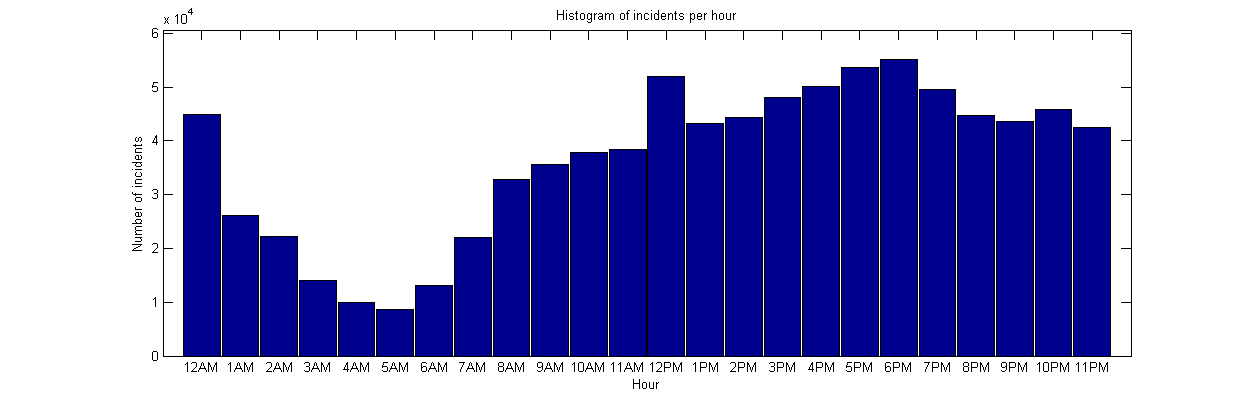
\includegraphics[scale=0.7]{histogram_hours}
	\\\\\\
	Here we can see the number of incidents that occur at each hour of the day. There is a clear drop in the number of incidents as the night progresses, steadily rising through the morning. At around lunch time the number of incidents spikes drastically, then falls again. After that the number of incidents steadily rises until the peak at 6PM, then begins to fall.
	\\\\
	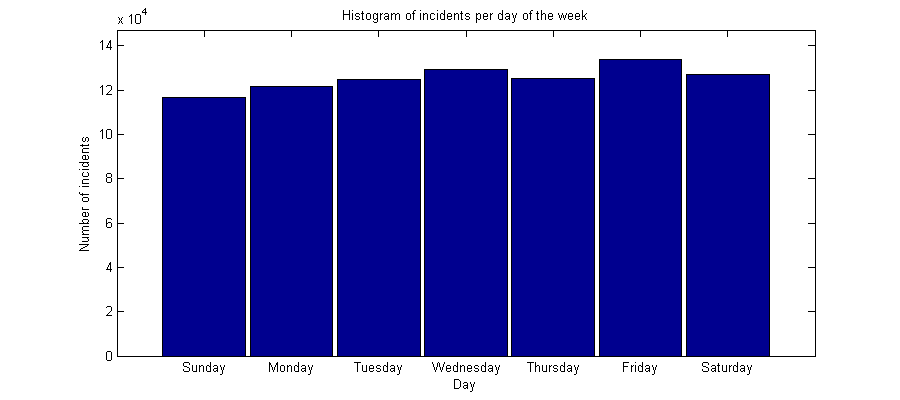
\includegraphics[scale=0.7]{histogram_days}
	\\\\
	Here we have the distribution of the number of incidents each day. There is a slight bump in the number of incidents on Friday, but there are no significant changes.
	\\\\\\
	\hspace*{-3cm}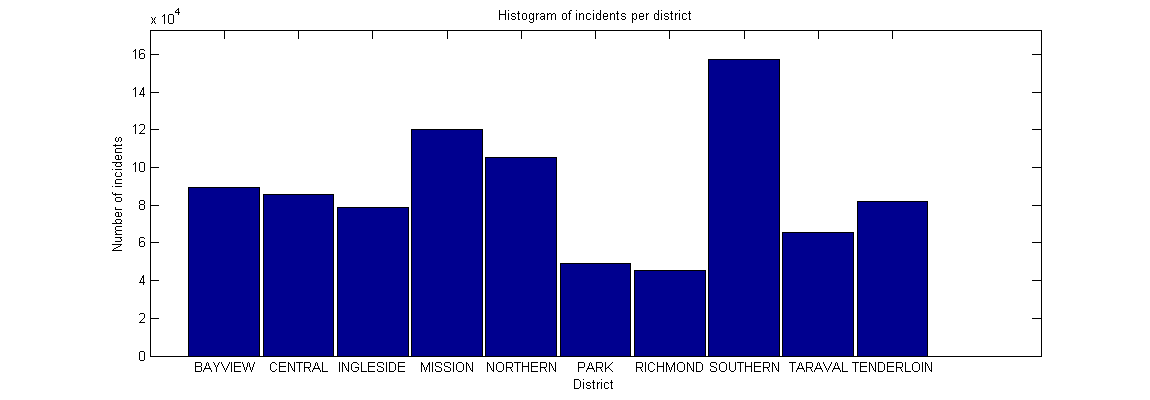
\includegraphics[scale=0.7]{histogram_district}
	\\\\
	This shows the distribution of the incidents in each district. The distribution shows which parts of the city may be more dangerous. 
	\\\\\\
	The list of crimes with the hour they are most likely to occur.\\\\
	\hspace*{3.5cm}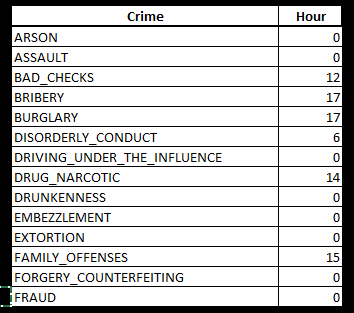
\includegraphics{crimes_hours}
	\\
	\hspace*{3.5cm}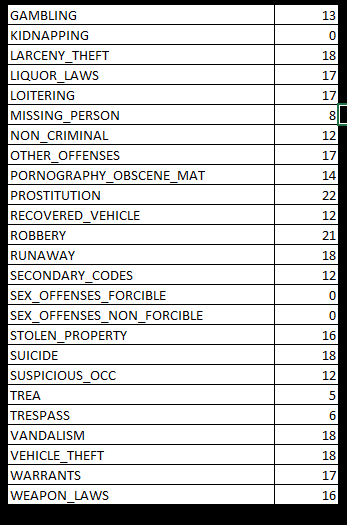
\includegraphics{crimes_hours_2}
	\\\\
	Here is the most likely hour that each crime is going to occur. The most likely hours that crimes occur are around 10PM, 0AM, 12PM, and 6PM.
	\\\\\\
	The crime most likely to occur in Bayiew is other offenses\\
	The crime most likely to occur in Central is larceny and theft\\
	The crime most likely to occur in Ingleside is other offenses\\
	The crime most likely to occur in Mission is other offenses\\
	The crime most likely to occur in Northern is larceny and theft\\
	The crime most likely to occur in Park is larceny and theft\\
	The crime most likely to occur in Richmond is larceny and theft\\
	The crime most likely to occur in Southern is larceny and theft\\
	The crime most likely to occur in Taraval is larceny and theft\\
	The crime most likely to occur in Tenderloin is drug and narcotic
	\\\\From this spread, we can see that larceny and theft is the most likely incident that occurs in many regions.
	
	\newpage
	\subsection{Part b}
	
	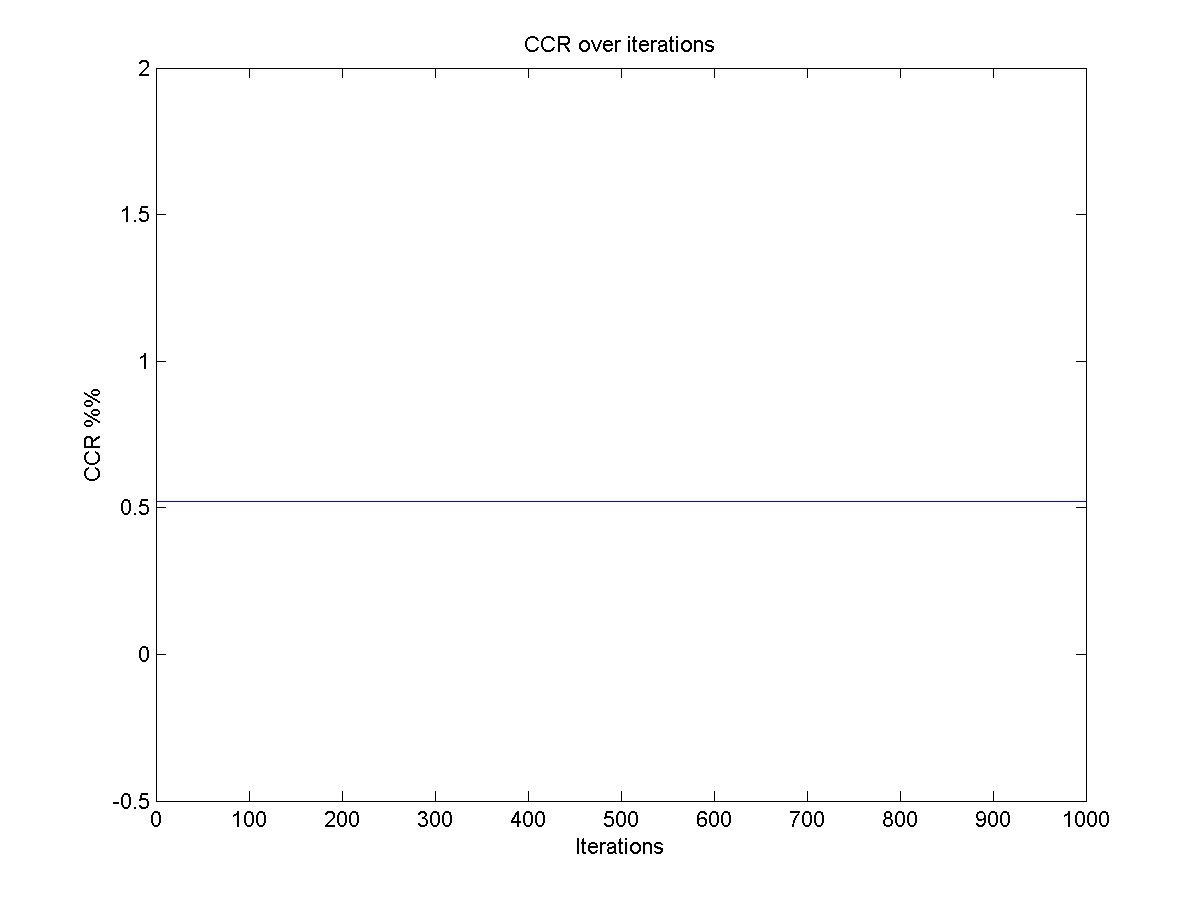
\includegraphics[scale=.8]{CCR}
	\\\\
	This graph indicates that the CCR rate did not noticeably change over the different iterations of the parameters. Unfortunately, this also indicates the CCR rate was very low for the experiment. The end result was only .5\% correct detection.
	\\\\\\
	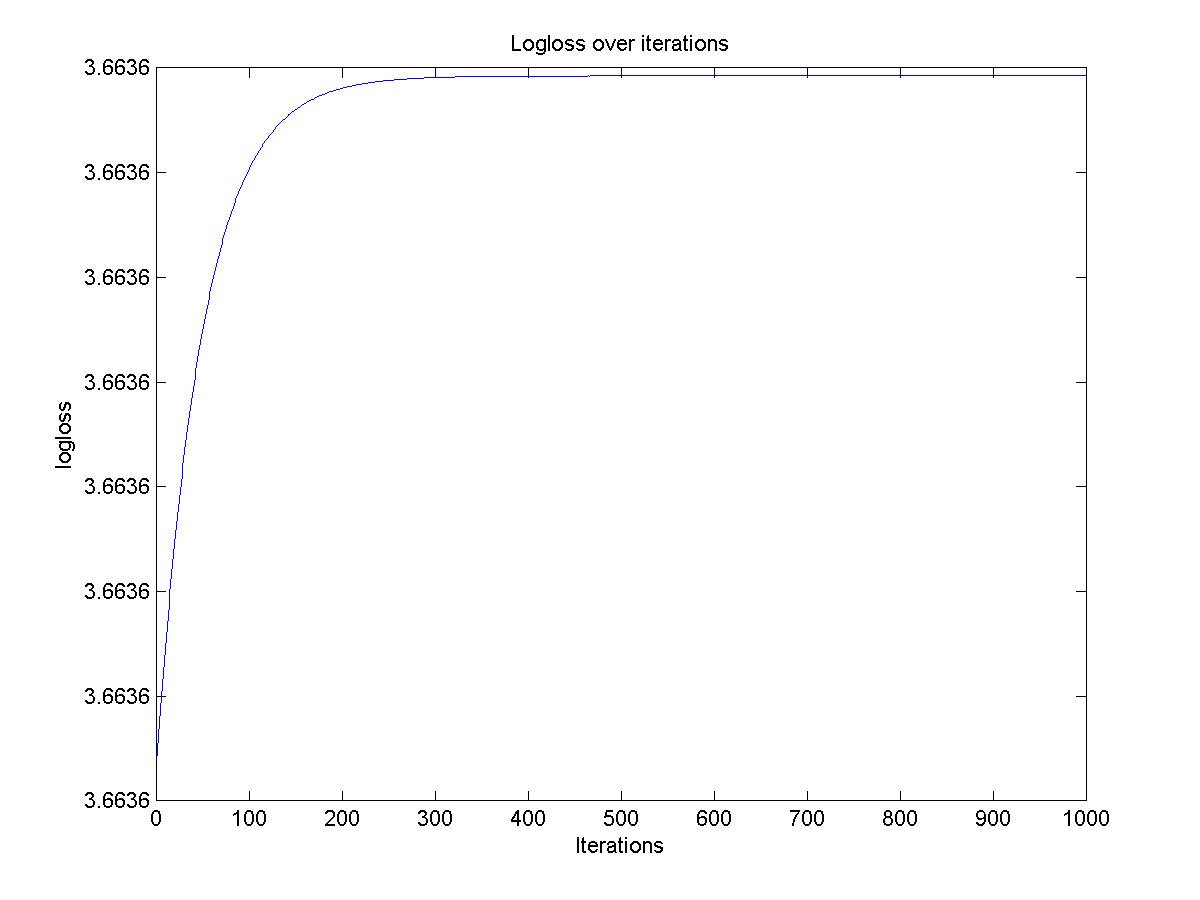
\includegraphics[scale=0.8]{logloss}
	\\\\
	As iterations increase, the logloss value approaches an asymptote of around 3.6636, and levels off.

	\newpage
	\subsection{Part c}

	\newpage
	%----------------------------------------------------------------------------------------
	%	PROBLEM 2
	%----------------------------------------------------------------------------------------
	
	\section{SVM Classifier for Text Documents}
	
	\subsection{Part a}
	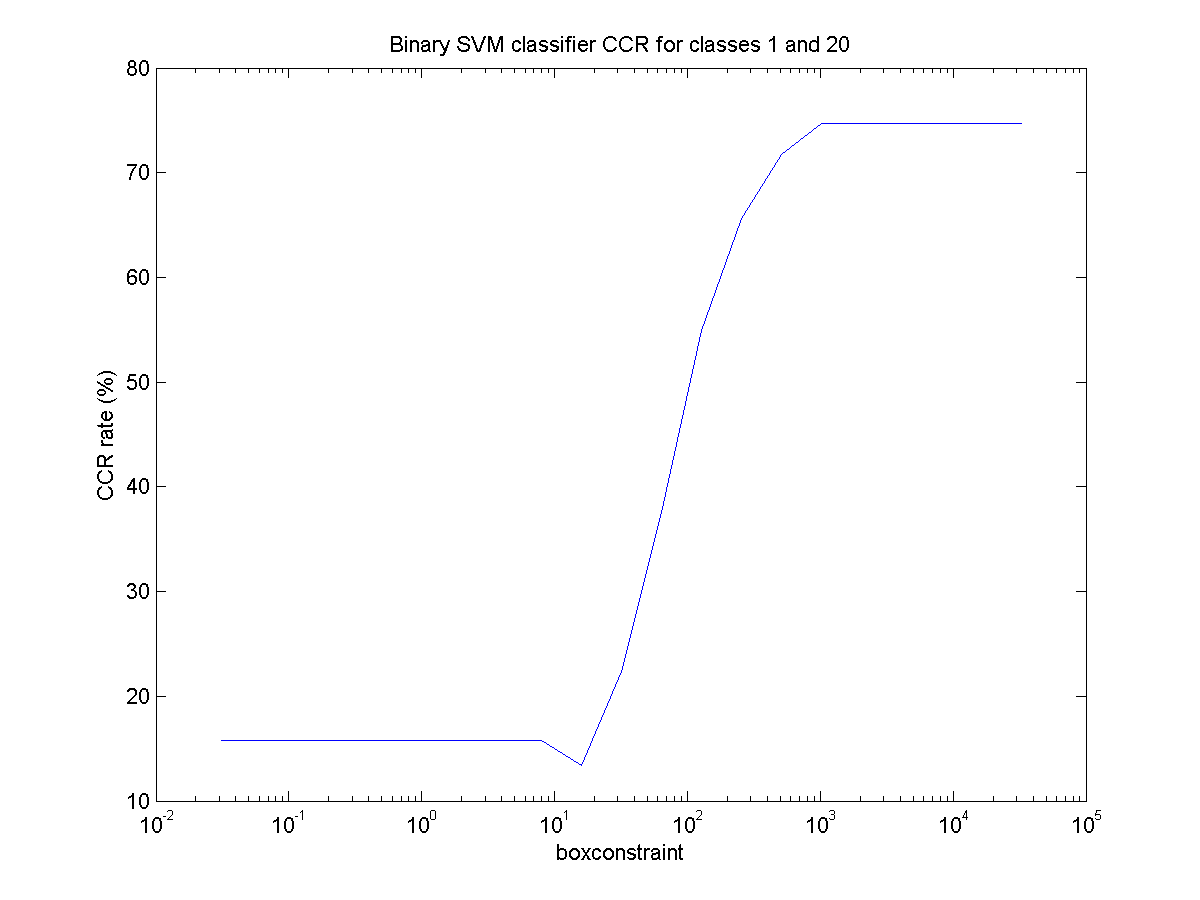
\includegraphics[scale=.8]{part_a_CV_CCR}
	\\\\
	The best CCR was 80.32\% which was achieved when $C^*=2^{10}$. This can be clearly seen from the curve, where the CCR rate increases with boxconstraint. Eventually it hits a plateau value, after which boxconstraint does not improve the CCR.
	\newpage

	\subsection{Part b}
	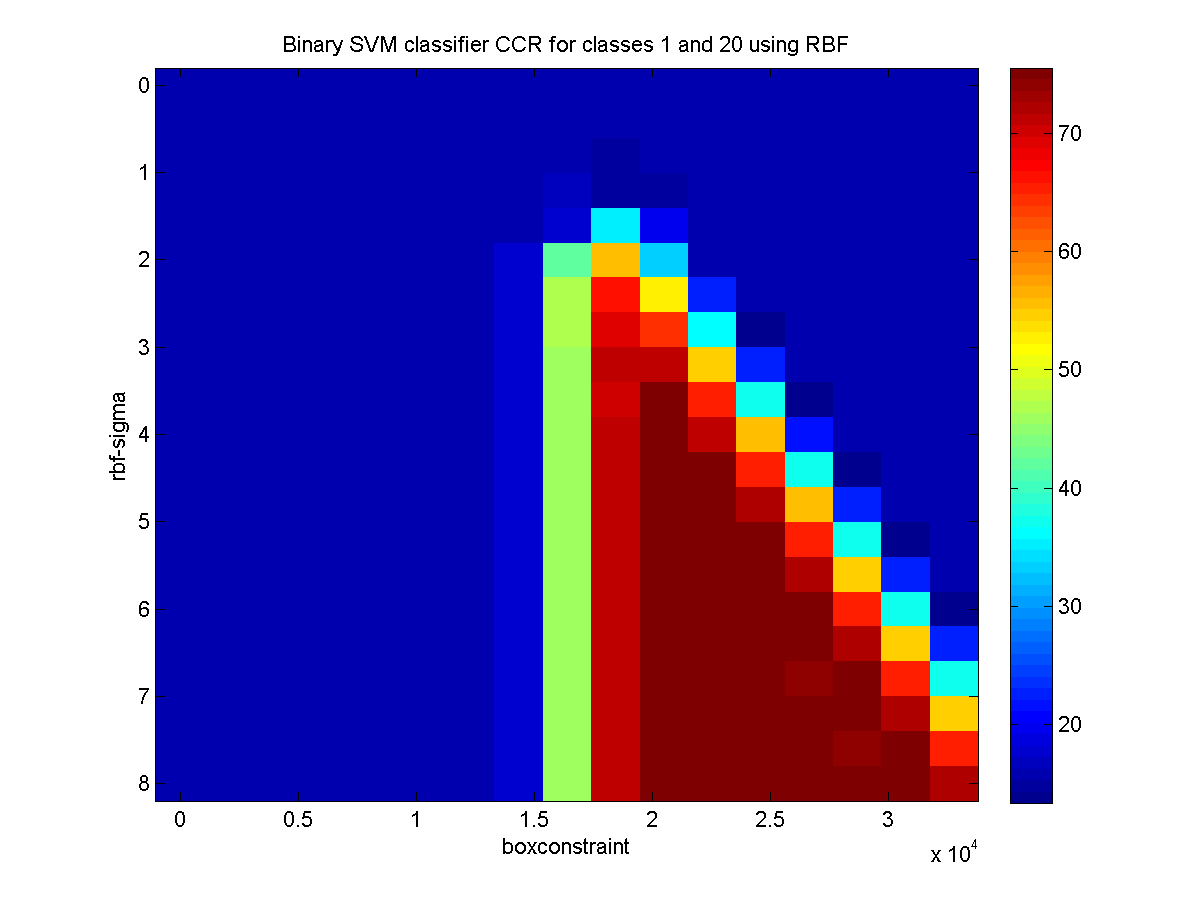
\includegraphics[scale=.8]{part_b_CV_CCR}
	\\\\
	The best CCR was 79.44\% which was achieved when $C^* = 2^{11}$ and rbf-sigma=$2^{-3}$. The graph shows the region in which the combined boxconstraint and rbf-sigma values produce an increased CCR. Outside this region, the CCR drops dramatically.

	\newpage		
	\subsection{Part c}
	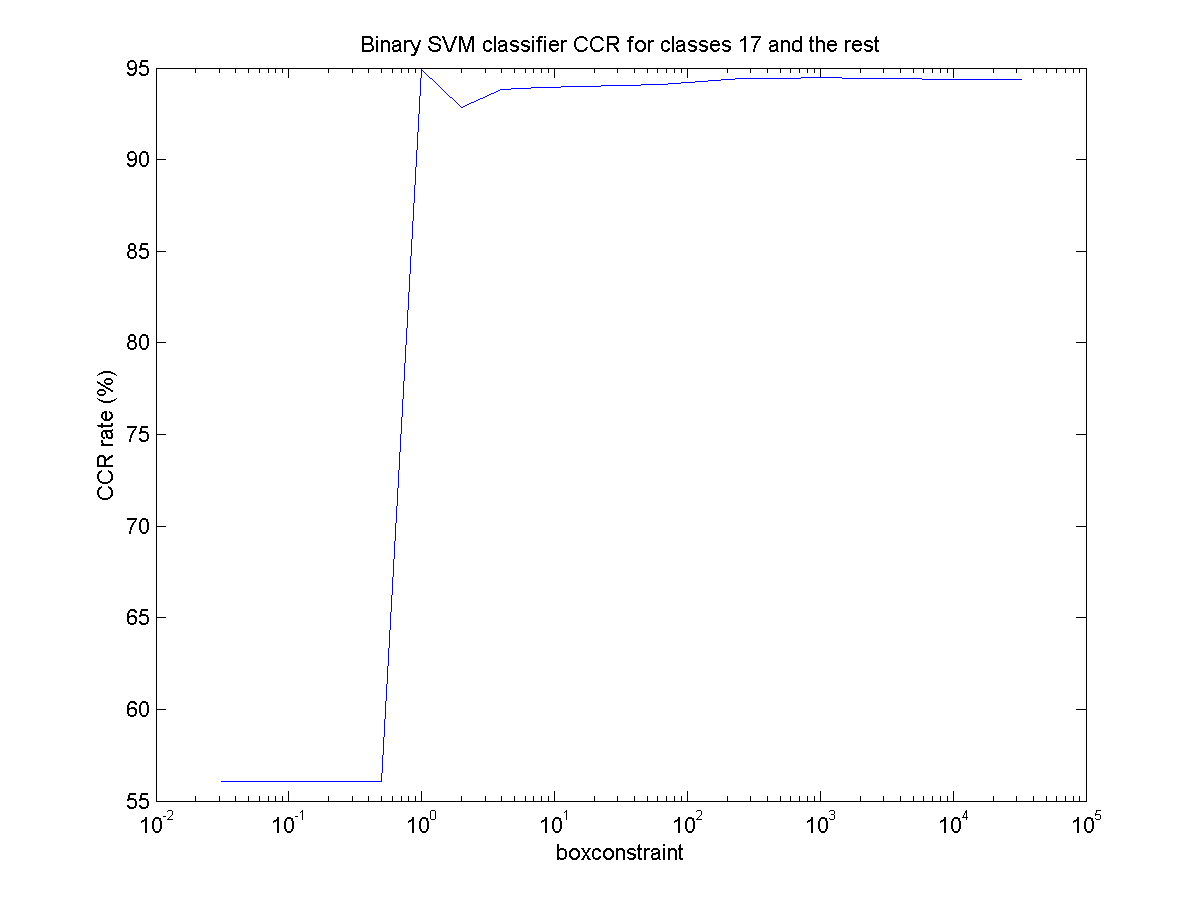
\includegraphics[scale=0.8]{part_c_CV_CCR}
	\\\\
	The best CCR was 95.78\% which was achieved when $C^* = 2^0$. The graph shows the sharp rise and peak as the boxconstraint rises, which then falls off after $C^*$.
	\\\\
	Confusion Matrix:
	\\\\
	\hspace*{3.5cm}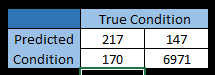
\includegraphics{part_c_confusion_matrix}
	\\\\
	In the confusion matrix it is clear that there are many more negative samples than positive ones, however, the vast majority have been properly classified as being not class 17. The accuracy of this classification is likely due to the sheer number of negative samples which allow for accurate prediction.
	
	\newpage
	\subsection{Part d}
	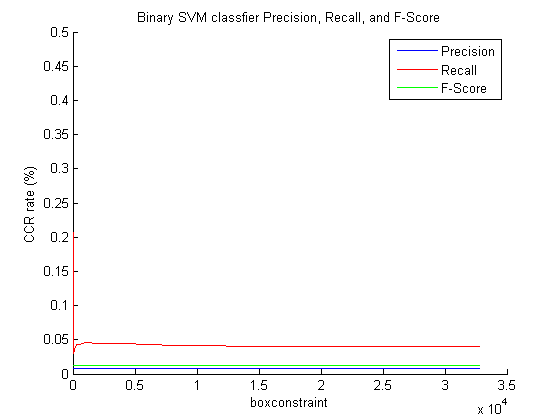
\includegraphics[scale=0.8]{part_d_CV_CCR}
	\\\\
	Best value of C as determined by the precision and the F-score is $2^0$. In the graph we can see the recall and precision, and in turn the F-score values are fairly constant throughout the different boxconstraint values.
	\\\\
	Confusion Matrix:
	\\\\
	\hspace*{4cm}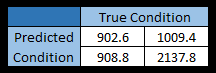
\includegraphics{part_d_confusion_matrix}
	\\\\
	Since the best F-score and precision value occur at the same value of the boxconstraint, there is one confusion matrix. As can be seen there is a large amount of misclassification, and only the classification of samples as not being in class 17 can be said to be more accurate. This seems to indicate that using the CCR as the determinant of the optimal $C^*$ value is the correct approach.
	
	\newpage
	
	\subsection{Part e}
	The overall CCR is 31.55\%. This can likely be improved with a better boxconstraint. The training time was 100.68s, and the testing time was 98.48s. 
	\\\\
	The confusion matrix is:
	\\\\
	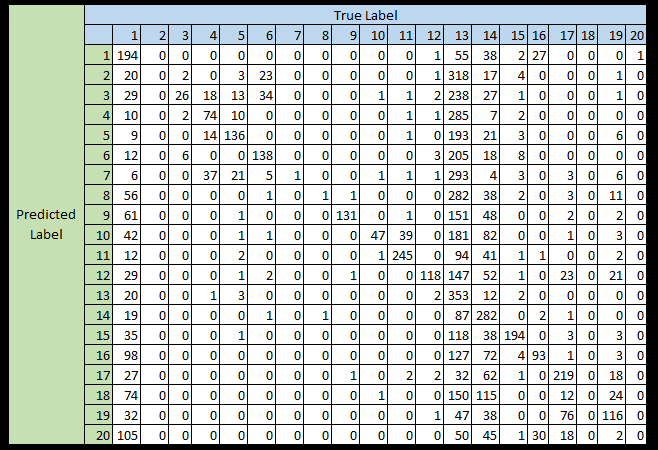
\includegraphics{part_e_confusion_matrix}
	
	\newpage
	\subsection{Part f}
	The overall CCR is 30.33\%. The training time was 83.31s, and the testing time was 201.37s.
	\\\\
	The confusion matrix is:
	\\\\
	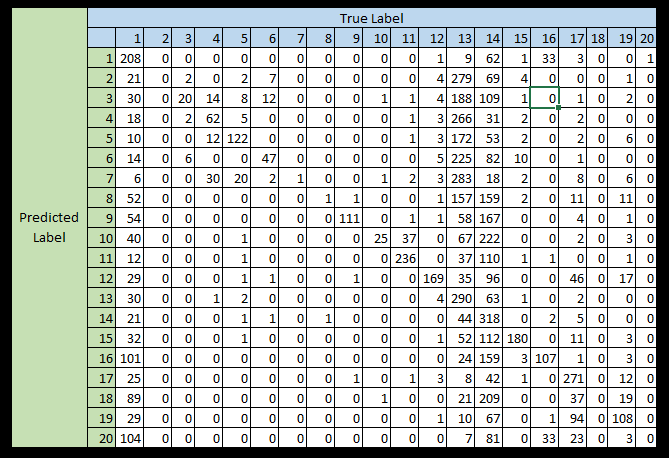
\includegraphics{part_f_confusion_matrix}
	
\end{document}